\documentclass[tikz]{standalone}

\usepackage[utf8]{inputenc}
\usepackage[T1]{fontenc}
\usepackage{cmap}
\usepackage{amsmath}
\usepackage{amssymb}
\usepackage{verbatim}
\usepackage{bm}

\renewcommand{\familydefault}{\sfdefault}
\usepackage[cm]{sfmath}

\usetikzlibrary{bending}
\usetikzlibrary{decorations.pathreplacing}
\usetikzlibrary{decorations.pathmorphing}
\usetikzlibrary{fadings}
\usetikzlibrary{shapes}

\definecolor{cblue}{rgb}{0.122, 0.467, 0.706}

\begin{document}
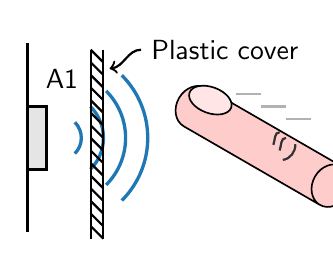
\begin{tikzpicture}[scale=0.8]

\draw[draw=none, use as bounding box] (0, 0.25) rectangle (4.4, -3.25);

\draw [very thick] (0, 0) -- (0, -3);
\draw [fill=black!10, thick] (0, -1) rectangle ++(0.3, -1);
\draw [cblue, very thick, decoration=expanding waves, segment length=8pt, decorate] (0.5, -1.5) -- ++(1.6, 0);
\node [above right=3pt] at (0, -1) {A1};

\draw [thick] (1.0, -0.1) -- ++(0, -3);
\draw [thick] (1.2, -0.1) -- ++(0, -3);
\foreach \y in {0, ..., 14}
    \draw [thick] (1.0, {-\y*0.2 - 0.1}) ++(0, 0) -- ++(0.2, -0.2);
\draw [thick, <-] (1.2, -.5) ++(0.1, 0.1) to [out=0, in=180] ++(0.5, 0.3) node[right, text width=70pt]{Plastic cover};

\node [color=black, fill=red!20, semithick, cylinder, rotate=-30, draw, aspect=1.99, minimum height=70pt, minimum width=16pt]
      at (3.5, -1.5) {};
\node [color=black, fill=red!10, semithick, ellipse, rotate=-20, draw, minimum height = 7pt, minimum width = 16pt]
	at (2.9, -0.9) {} ;

\draw [thick, black!80] (3.9, -1.61) to [out=70, in=180] ++(0.1, 0.2);
\draw [thick, black!80] (4.0, -1.7) to [out=70, in=180] ++(0.1, 0.2);
\draw [thick, black!80] (4.05, -1.85) to [out=10, in=270] ++(0.2, 0.25);
\foreach \y in {0, ..., 2}
    \draw [thick, black!30] (4.1 - 0.4*\y, -1.2+0.2*\y) -- ++(0.4, 0);
\end{tikzpicture}
\end{document}
